\documentclass[tikz,border=2pt]{standalone}
\usepackage{amsmath,amssymb}
\usepackage{tikz}
\usetikzlibrary{arrows.meta}

\begin{document}
% LOTP inside the conditional world C (a rainy day): routes B1, B2 with P(B1 | C) = 0.7 and
% delay probabilities 0.2 and 0.5; every probability in the tree is conditional on C.
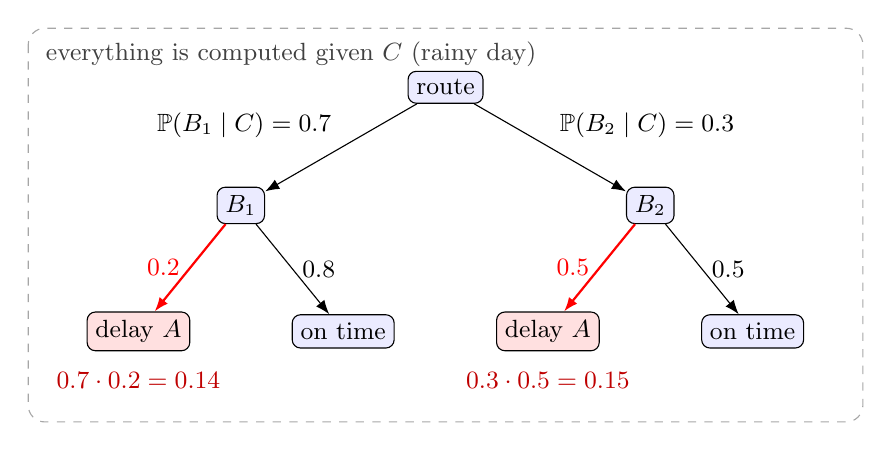
\begin{tikzpicture}[every node/.style={font=\small}, >={Latex[length=1.8mm]}, lvl/.style={draw, rounded corners=3pt, fill=blue!8, inner sep=3pt}]
	\draw[gray!70, dashed, rounded corners=6pt] (-5.3,0.75) rectangle (5.3,-4.25);
	\node[gray!50!black, anchor=north west, font=\small] at (-5.2,0.7) {everything is computed given $C$ (rainy day)};
	\node[lvl] (root) at (0,0) {route};
	\node[lvl] (B1) at (-2.6,-1.5) {$B_1$};
	\node[lvl] (B2) at (2.6,-1.5) {$B_2$};
	\draw[->] (root) -- (B1) node[midway, above left, font=\small] {$\mathbb{P}(B_1\mid C)=0.7$};
	\draw[->] (root) -- (B2) node[midway, above right, font=\small] {$\mathbb{P}(B_2\mid C)=0.3$};
	\node[lvl, fill=red!12] (A1) at (-3.9,-3.1) {delay $A$};
	\node[lvl] (N1) at (-1.3,-3.1) {on time};
	\node[lvl, fill=red!12] (A2) at (1.3,-3.1) {delay $A$};
	\node[lvl] (N2) at (3.9,-3.1) {on time};
	\draw[->, red, thick] (B1) -- (A1) node[midway, left, font=\small, red] {$0.2$};
	\draw[->] (B1) -- (N1) node[midway, right, font=\small] {$0.8$};
	\draw[->, red, thick] (B2) -- (A2) node[midway, left, font=\small, red] {$0.5$};
	\draw[->] (B2) -- (N2) node[midway, right, font=\small] {$0.5$};
	\node[red!75!black, font=\small, anchor=north] at (-3.9,-3.5) {$0.7\cdot0.2=0.14$};
	\node[red!75!black, font=\small, anchor=north] at (1.3,-3.5) {$0.3\cdot0.5=0.15$};
	
\end{tikzpicture}
\end{document}
